\documentclass[12pt]{article}
\usepackage{graphicx}
\usepackage{amsmath}
\usepackage{hyperref}
\usepackage{geometry}
\usepackage{listings}
\usepackage{caption}
\usepackage{float}
\geometry{a4paper, margin=1in}

\title{MPI Performance and Scaling Study}
\author{Weixiao Zhan}
\date{\today}

\begin{document}

\maketitle
\section*{Aliev-Panfilov cardiac simulation}
Aliev-Panfilov cardiac equations describe the signal propagation in cardiac tissue.
$$
\begin{aligned}
    \frac{\partial e}{\partial t} 
        &= \delta \nabla^2 e - ke(e - a)(e - 1) - er 
        & \text{on } \Omega_T \\
    \frac{\partial r}{\partial t} 
        &= -\left[\varepsilon + \frac{\mu_1 r}{\mu_2 + e}\right] \left[r + ke(e - b - 1)\right]
        & \text{on } \Omega_T, \\
    \vec{n} \cdot \delta \nabla e 
        &= 0 \quad \text{on } \partial \Omega \\
    (e, r)_{t=0} 
        &= (e(\cdot, 0), r(\cdot, 0))
\end{aligned}
$$

Listing \ref{lst:pseudocode} shows the pseudo-code for numerical computation  
for above differential equations,
in which, $E, E_p, R$ are three $[(m+2) \times (n+2)]$ size matrices.

\begin{minipage}{\textwidth}
\centering
\begin{lstlisting}[language=C]
For a specified number of iterations
for (j=1; j < m+1; j++) {
for (i=1; i < n+1; i++) {
    // NOT a PDE solver, but calculating the Laplace operator
    E[j,i] = E_p[j,i] + alpha*(  E_p[j,i+1] + E_p[j,i-1] 
                               + E_p[j+1,i] + E_p[j-1,i] 
                               - 4 * E_p[j,i]); 
    // ODE SOLVER
    E[j,i] += -dt * (kk * E_p[j,i] * (E_p[j,i]-a) 
                  * (E_p[j,i]-1) + E_p[j,i] * R[j,i]);
    R[j,i] +=  dt * (eps+M1* R[j,i]/(E_p[j,i]+M2))
                  * (-R[j,i]-kk*E_p[j,i]*(E_p[j,i]-b-1));
}}
swap E_p and E
End repeat
\end{lstlisting}
\captionof{lstlisting}{Pseudocode for numerical simulation}
\label{lst:pseudocode}
\end{minipage}

\section{Development Flow}
The Aliev-Panfilov cardiac simulation program has simple data dependency.
thus can be scaled to multi-processes using MPI library.

\subsection{Program Description}
There are three stages in simulation program, called apf, execution:
init, solve, and reduce.
The over Memory layout of one matrix is shown in Figure \ref{fig:layout}.

\begin{figure}[h]
    \centering
    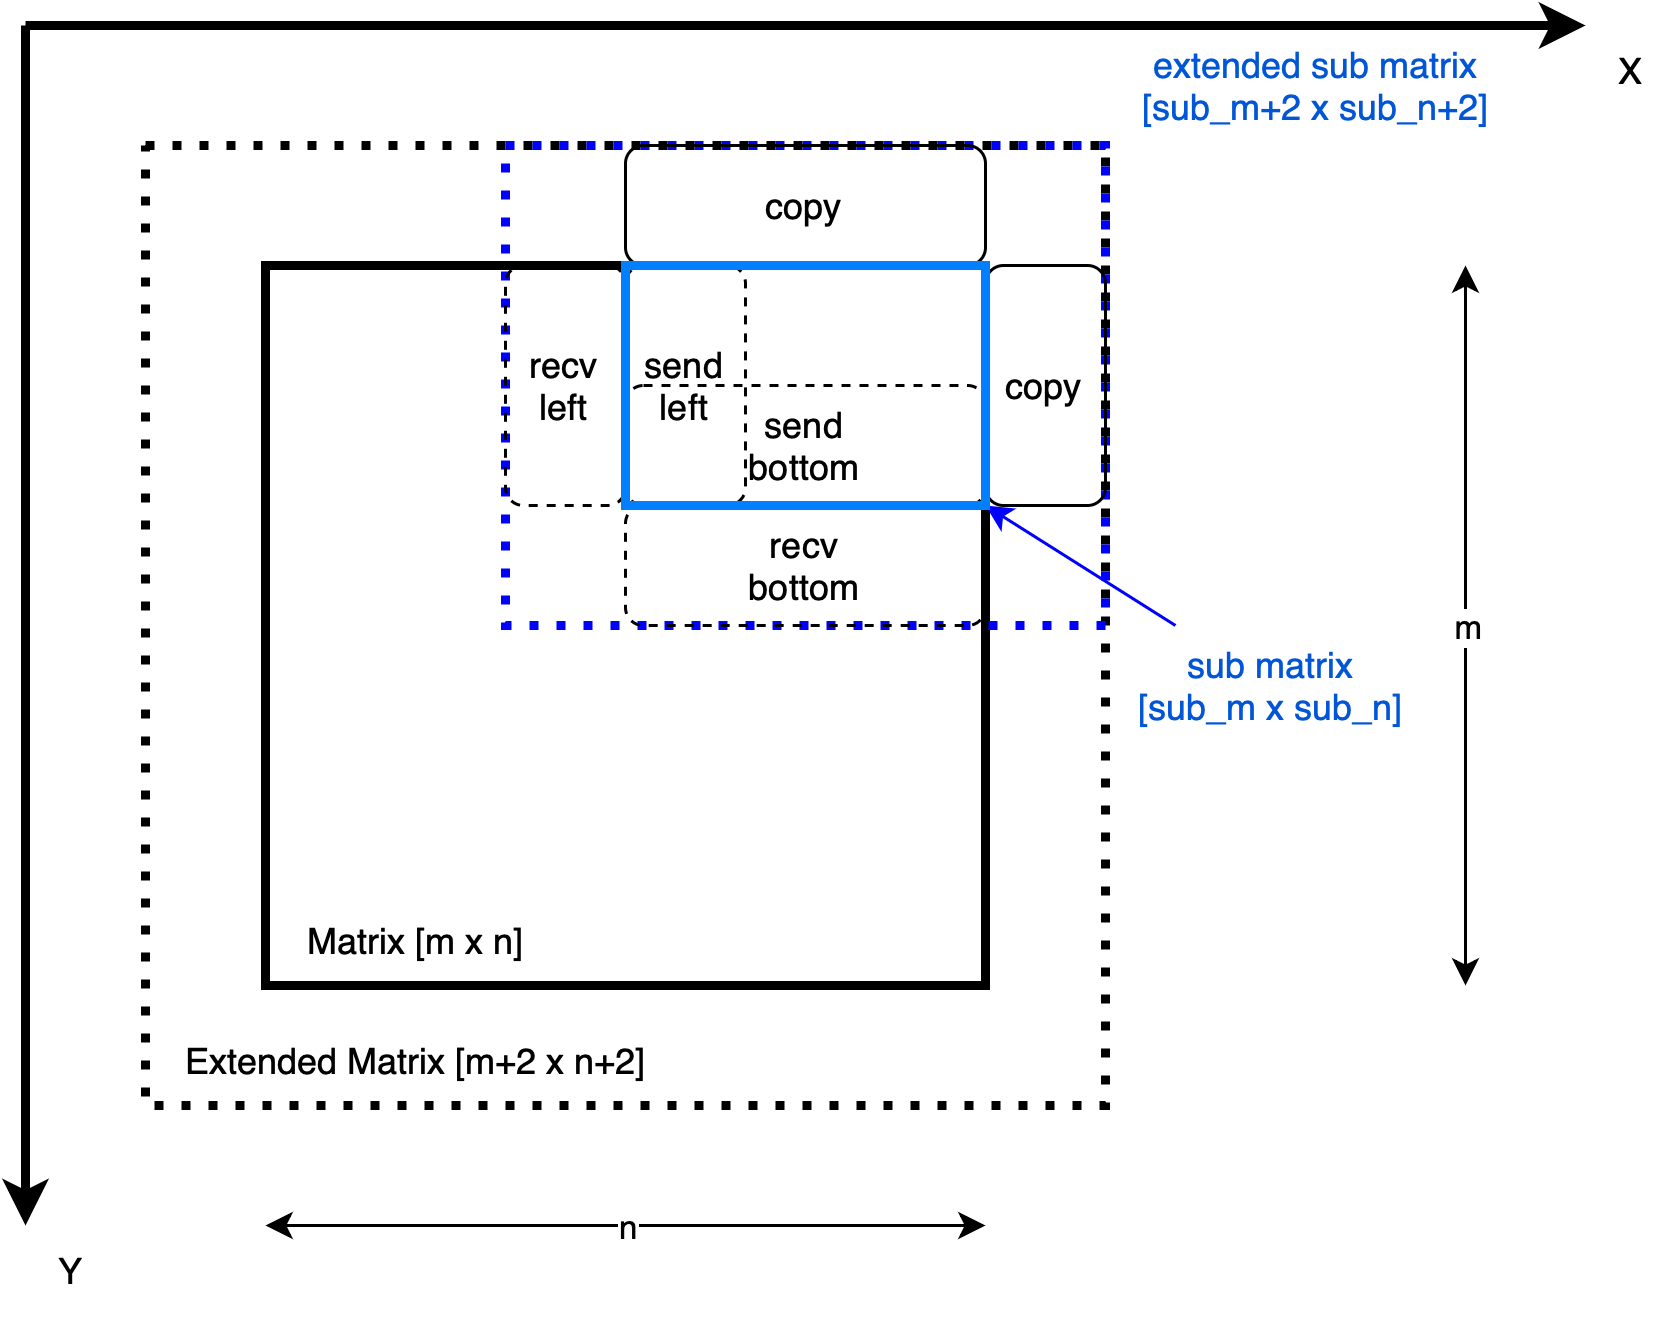
\includegraphics[width=0.8\textwidth]{img/layout.png}
    \caption{layout}
    \label{fig:layout}
\end{figure}

\subsubsection{init}
The main process initialize extended matrix of $E_p$ and $R$ with starting conditions;
then uses MPI to distribute extended sub matrices to their corresponding working processes.

\subsubsection{solve}
For every iteration, 
each process first exchange ghost sells of $E_p$ with their neighbor processes.
Specifically, the process need to pack the left and right cells its needs to send
and unpack the received left and right ghost cells.
Top and bottom ones can be sent and received in place as the matrices are stored in row major order.
The exchange of ghost cells are using non-blocking MPI to reduce waiting.
If the process is on the edge, the ghost sells are copy updated by the row or column that are 2 cells away.

After ghost cell exchange, each process perform the numerical computation shown in Listing \ref{lst:pseudocode} to solve the PED.
The numerical computation along with some of the packing and unpacking routine are vectorized using compiler hints.

\subsubsection{reduce}
After or during the simulation, the program might need to gather results to one process.
The program supports reducing two types of results.

One is gathering all sub matrices of $E$ to reconstruct the full matrix of $E$,
which can be helpful for plotting and downstream computation that requires the full simulation results.
This is achieved by regular MPI send and receive routine.

The other is just gathering $L_\infty$ and $L_2$ norm of $E$,
which can be helpful for correctness check and save bandwidth.
This is achieved by \texttt{MPI\_Reduce} with max and sum reduce operator respectively.

\subsection{Development Process}
\begin{enumerate}
    \item Implement initial distribution routine;
    \item Implement ghost cell exchange routine;
    \item Change numerical simulation code to tile loop (hoping to improved cache hit rate);
    \item Implement reduce routine;
    \item Change numerical simulation code to use SIMD;
    \item Change ghost cell exchange routine to use SIMD;
    \item Batch jobscript for N0, N1, N2.
\end{enumerate}


\subsection{Performance Improvements}
Along the development process, the perform are measured at $m=n=800$ with $4\times4$ process grid on a local machine.
The performance improvements are shown in Figure \ref{fig:pi}.
The multi-processing and SIMD improved performance.

\begin{figure}[h]
    \centering
    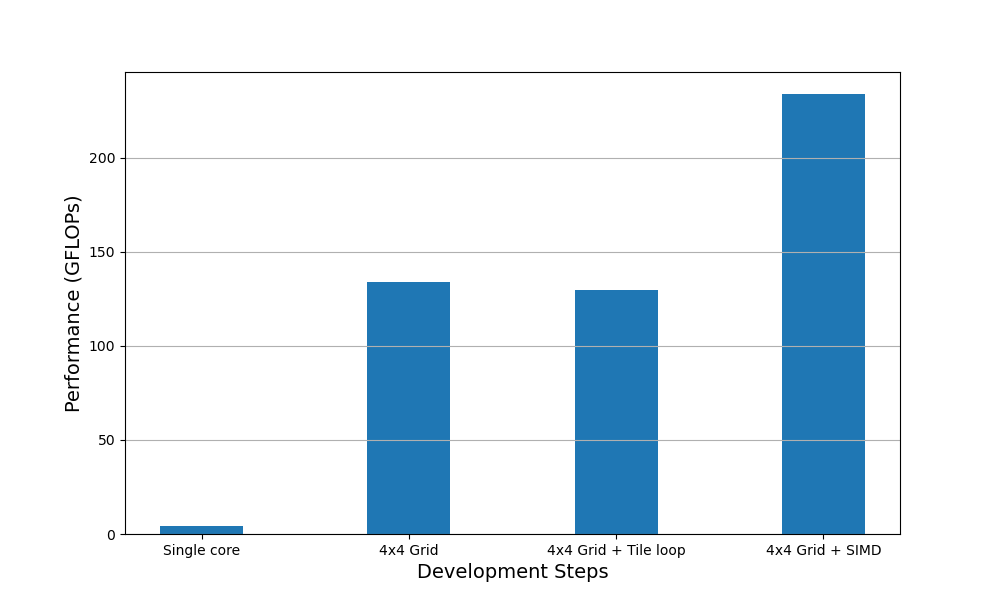
\includegraphics[width=0.8\textwidth]{img/pi.png}
    \caption{Performance Implements}
    \label{fig:pi}
\end{figure}

\section{Results}

\subsection{Single Processor Performance}
Figure \ref{fig:N0} shows the peak performance reached at N0 problem size.

MPI overhead caused $-0.3\%, 4.4\%, 3.7\%, 8.5\%, 13\%, 20\%$ of performance loss
on $1,2,4,8,12,16$ processes respectively. 
At 16 processes, 6\% out of 20\% performance drop comes from computation.
Reminder 14\% comes from other non-communication overhead. 

The most significant non-communication overhead is repeated ghost updates.
In no communication implementation, 
all processes consider them as edge processes
and copy update its ghost cells in every iteration. 
In no MPI version, the number of ghost cell is 
the circumference of matrices $ = O(2m + 2n)$.
Whereas in multi processes, the number of ghost cell is 
number of processes * circumference of each sub matrices $ = O(2(m\cdot py+n \cdot px))$
The more processes in the program, more computation spent on ghost cell updates.

\begin{figure}[h]
    \centering
    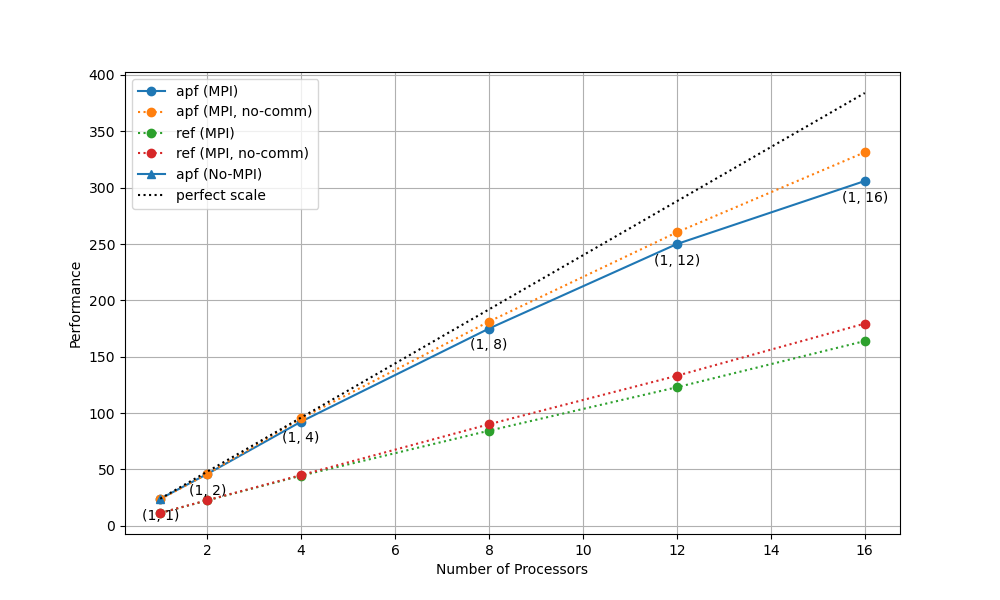
\includegraphics[width=\textwidth]{img/N0.png}
    \caption{Singe Processor Processor}
    \label{fig:N0}
\end{figure}

\subsection{Strong Scaling Study (1-16 cores)}
Figure \ref{fig:N0-scale} shows the speedup and efficiency of the program on N0 problem size.
The figure might have suggested my apf program scale less efficiently.
However, the true factor is the base lines performance.
My apf program would skipped unnecessary MPI routines 
when running in 1 MPI process, 
, leading to a higher base line.
Thus despite the scale efficiency is lower,
my program runs significantly faster than reference program on all process numbers.

\begin{figure}[h]
    \centering
    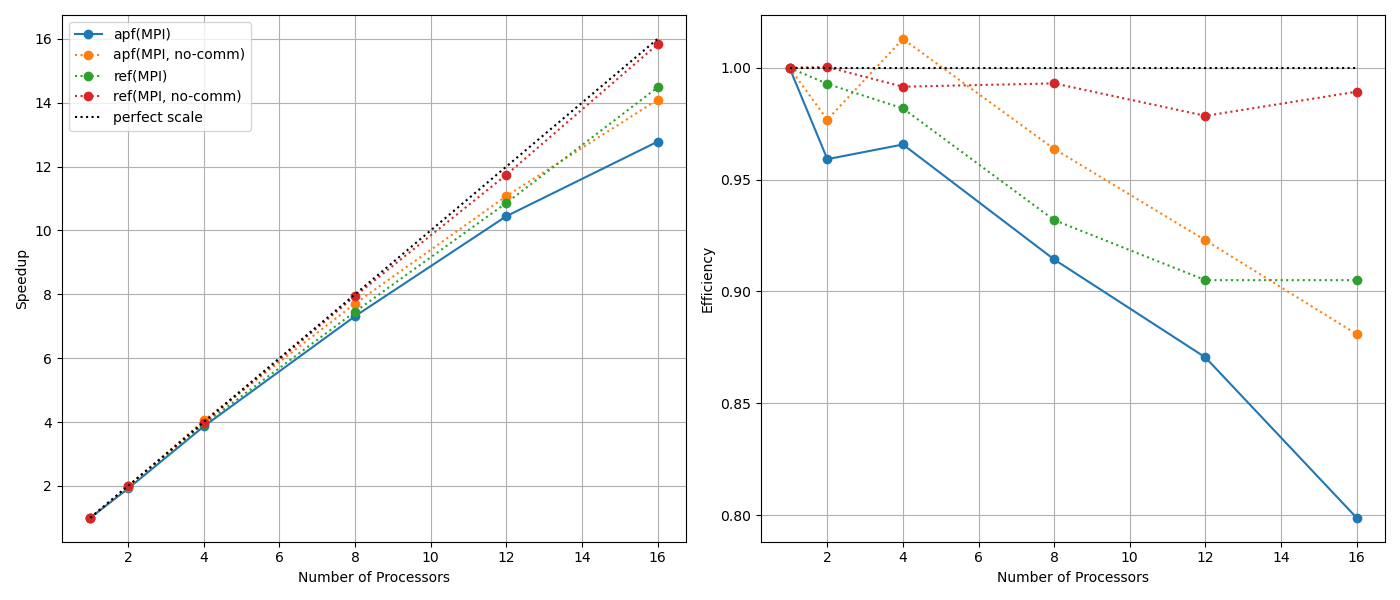
\includegraphics[width=\textwidth]{img/N0_scale.png}
    \caption{N0 scale study}
    \label{fig:N0-scale}
\end{figure}

\subsection{Strong Scaling Study (16-128 cores)}
Table \ref{tab:N1}, Figure \ref{fig:N1} and Figure \ref{fig:N1-scale} 
shows the peak performance and scale efficiency at N1 problem size.

From 16 to 64 processes, the program gradually use up all cores on one AMD EPYC Processor.
At 128 processes, the program takes up one entire node with two CPU socket
and the MPI is communicating between Non-Uniform Memory (NUM).
Despite the memory been different,
MPI communication caused 14.7\% of performance decrease at 64 processes,  
and 15.2\% at 128 processes, which are fairly close, suggesting 
socket bus is not limiting the scalability of the program.

Figure \ref{fig:N1-scale} shows the scale efficiency of the program on N1 sized problem.
Similar to N0 scale result, my apf has better performance than reference program at all processes sizes.
The scale efficiency is lower due to better baseline result.
Suggesting some optimization employed by my apf program become less effective 
as the number of processes increases.

\begin{table}[h!]
\centering
\begin{tabular}{|c|c|c|}
\hline
\textbf{Processes} & \textbf{Geometry} & \textbf{GFlops} \\
\hline
16 & $8 \times 2$ & 381 \\
32 & $8 \times 4$ & 705 \\
64 & $8 \times 8$ & 1250 \\
128 & $8 \times 16$ & 1916 \\
\hline
\end{tabular}
\caption{N1 geometries}
\label{tab:N1}
\end{table}

\begin{figure}[h]
    \centering
    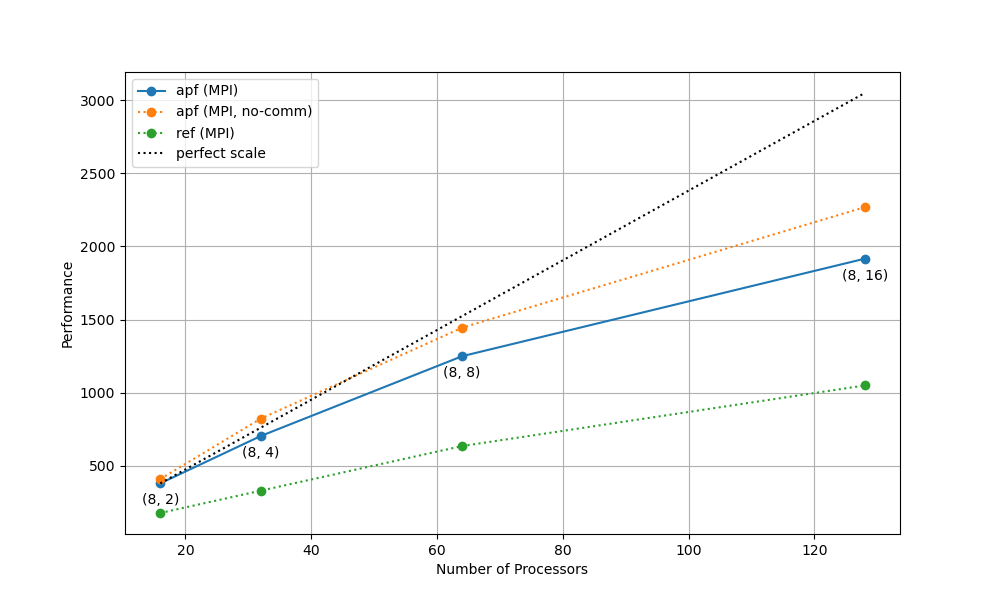
\includegraphics[width=0.8\textwidth]{img/N1.png}
    \caption{N1 performance}
    \label{fig:N1}
\end{figure}

\begin{figure}[h]
    \centering
    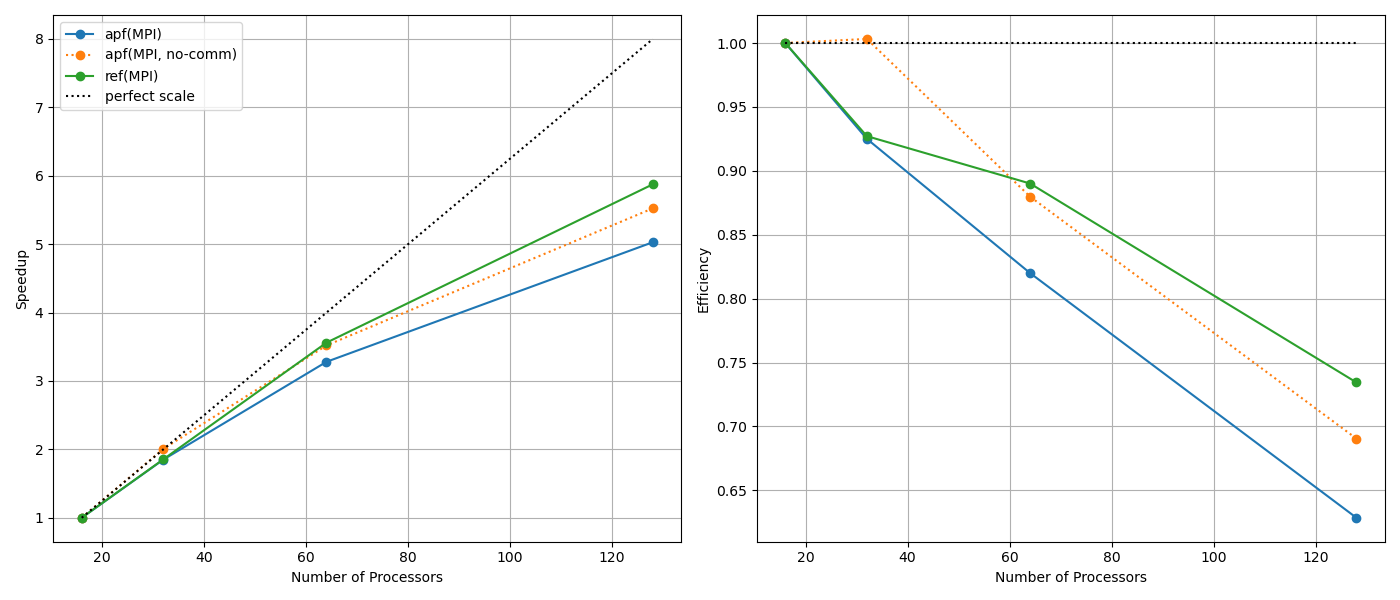
\includegraphics[width=\textwidth]{img/N1_scale.png}
    \caption{N1 scale study}
    \label{fig:N1-scale}
\end{figure}

\subsection{Large Core Count Performance Study}
Table \ref{tab:N2}, Figure \ref{fig:N2}, and Figure \ref{fig:N2-scale} 
shows the peak performance and scale efficiency at N2 problem size.
Doe to reference program is too slow, skip running them on N2.

Based on experience, the processes geometry should be around square and has slightly larger py.
Such geometries will results in near square and slightly wide sub matrices for each process.
Because the square sub matrices has the bast circumference to area ratio, 
they have the least ghost cell to exchange.
The wider sub matrices are also preferred, 
as top and bottom ghost cells can exchanged in place and no need to pack and unpack.

\begin{table}[h!]
\centering
\begin{tabular}{|c|c|c|}
\hline
\textbf{Processes} & \textbf{Geometry} & \textbf{GFlops} \\
\hline
128 & $8 \times 16$ & 360 \\
192 & $16 \times 12$ & 542 \\
256 & $4 \times 64$ & 601 \\
384 & $16 \times 24$ & 2109 \\
\hline
\end{tabular}
\caption{N2 geometries}
\label{tab:N2}
\end{table}

\begin{figure}[h]
    \centering
    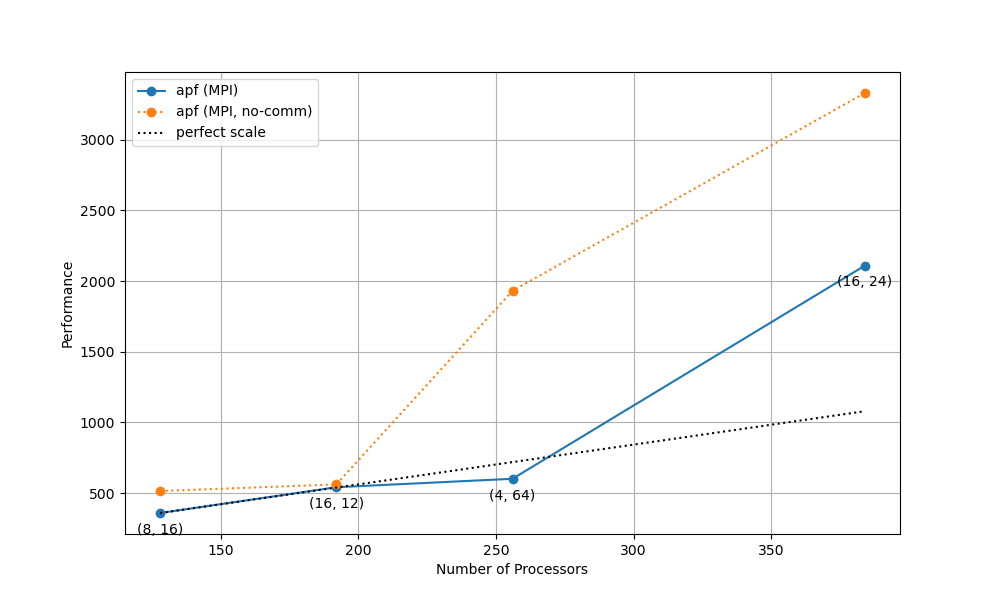
\includegraphics[width=0.8\textwidth]{img/N2.png}
    \caption{N2 performance}
    \label{fig:N2}
\end{figure}

\begin{figure}[h]
    \centering
    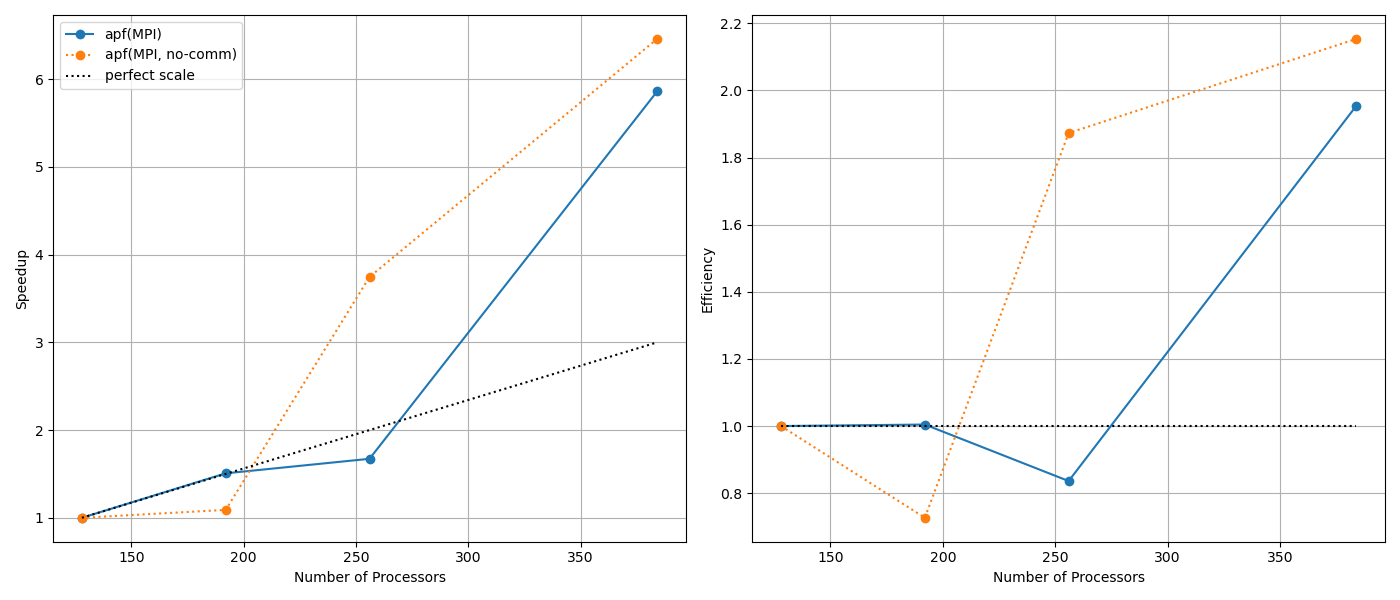
\includegraphics[width=\textwidth]{img/N2_scale.png}
    \caption{N2 scale study}
    \label{fig:N2-scale}
\end{figure}

\subsection{Communication Overhead Differences}
% \textbf{Q2.e) Explain the communication overhead differences observed between <=128 cores and >128 cores.}

For processes number less then 128, all processes nested on one node.
As discussed in previous sections, the communication cost didn't surge due to in-node NUMA.

From 128 to 384 process on N2,
the program spam on multiple nodes.
As shown in \ref{fig:N2}, some computation cost surged but some didn't.
I believe the cause is the processes are randomly distributed on different nodes,
Causing different number of ghost cell exchange happened between nodes.
Experiment also shows the performance on N2 vary significantly. 
And the variance could due to the random distribution of processes.

On a two nodes 256 processes program,
if the processes are distributed following their geometry,
the between-node communication can reduce by half in best case then worst case.

At 384 processes,
the remote direct memory access (RDMA) is automatically disabled.
MPI might have used a different routine for communication when RDMA is disabled.
Which could leads to the performance surge at 384 processes.

\subsection{Computation Cost}
Based on \ref{tab:computation-cost}, 384 processes yields best performance and lowest cost.

\begin{table}[h!]
\centering
\begin{tabular}{|c|c|}
\hline
\textbf{Processes} & \textbf{Computation cost} (SUs) \\
\hline
128 & 1.416 \\
256 & 1.410 \\
192 & 1.693 \\
384 & 0.725 \\
\hline
\end{tabular}
\caption{Computation cost}
\label{tab:computation-cost}
\end{table}

\section{Determining Geometry}

\subsection{Top-Performing Geometries}
At p=128, the top-performing geometries at N1 are $8\times 16$ and $16 \times 8$.

\subsection{Geometry Patterns}
The processes geometry should be around square and has slightly larger py.
Such geometries will results in near square and slightly wide sub matrices for each process.
Because the square sub matrices has the bast circumference to area ratio, 
they have the least ghost cell to exchange.
The wider sub matrices are also preferred, 
as top and bottom ghost cells can exchanged in place and no need to pack and unpack.

\section{Strong and Weak Scaling}

\subsection{Strong Scaling Comparisons}
% \textbf{Q4.a) Run your best N1 geometry (or as close as you can get) at 128, 192, 256, and 384 cores. Compare and graph your results from N1 and N2 for 128, 192, 256, and 384 cores.}
The results of best N1 geometries are shown in Table \ref{tab:N1} and Figure \ref{fig:N1}
The results of best N2 geometries are shown in Table \ref{tab:N2} and Figure \ref{fig:N2}

\subsection{Scaling Behavior}
% \textbf{Q4.b) Explain or hypothesize differences in the behavior of both strong scaling experiments for N1 and N2?}
The scaling behavior are shown in Figure \ref{fig:N1-scale} and Figure \ref{fig:N2-scale}
In summary, the program scale efficiency decrease as the number of process increases due to inevitable ghost cell communication and updates (discussed in previous sections).
When the number of process exceeds 128, i.e. the program is running on multiple node, the scale is much less efficient.

\section{Extra Credit}

\subsection{multi-processes plotting}
Shown in Figure \ref{fig:images_grid}, 
the program supports plotting when running with multi-processes.
The plotting process does not do computation. 

\begin{figure}[h]
    \centering
    \begin{minipage}[b]{0.45\textwidth}
        \centering
        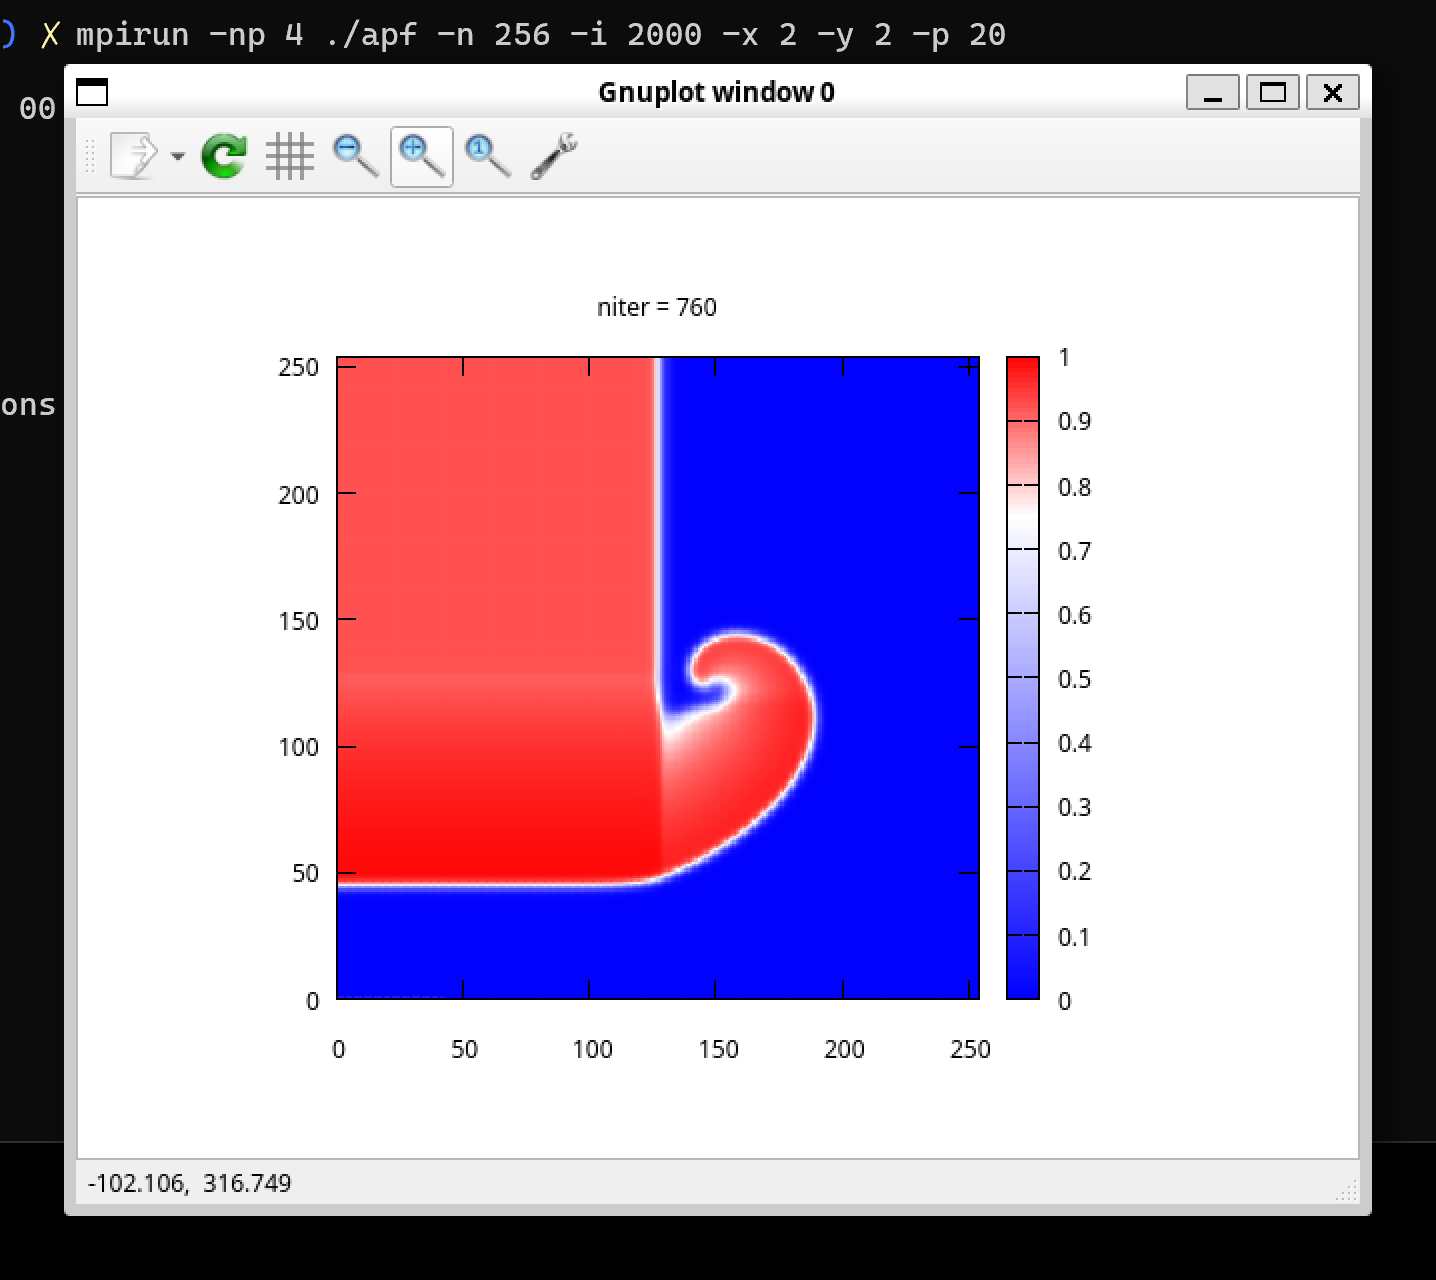
\includegraphics[width=\textwidth]{img/1.png}
    \end{minipage}
    \hfill
    \begin{minipage}[b]{0.45\textwidth}
        \centering
        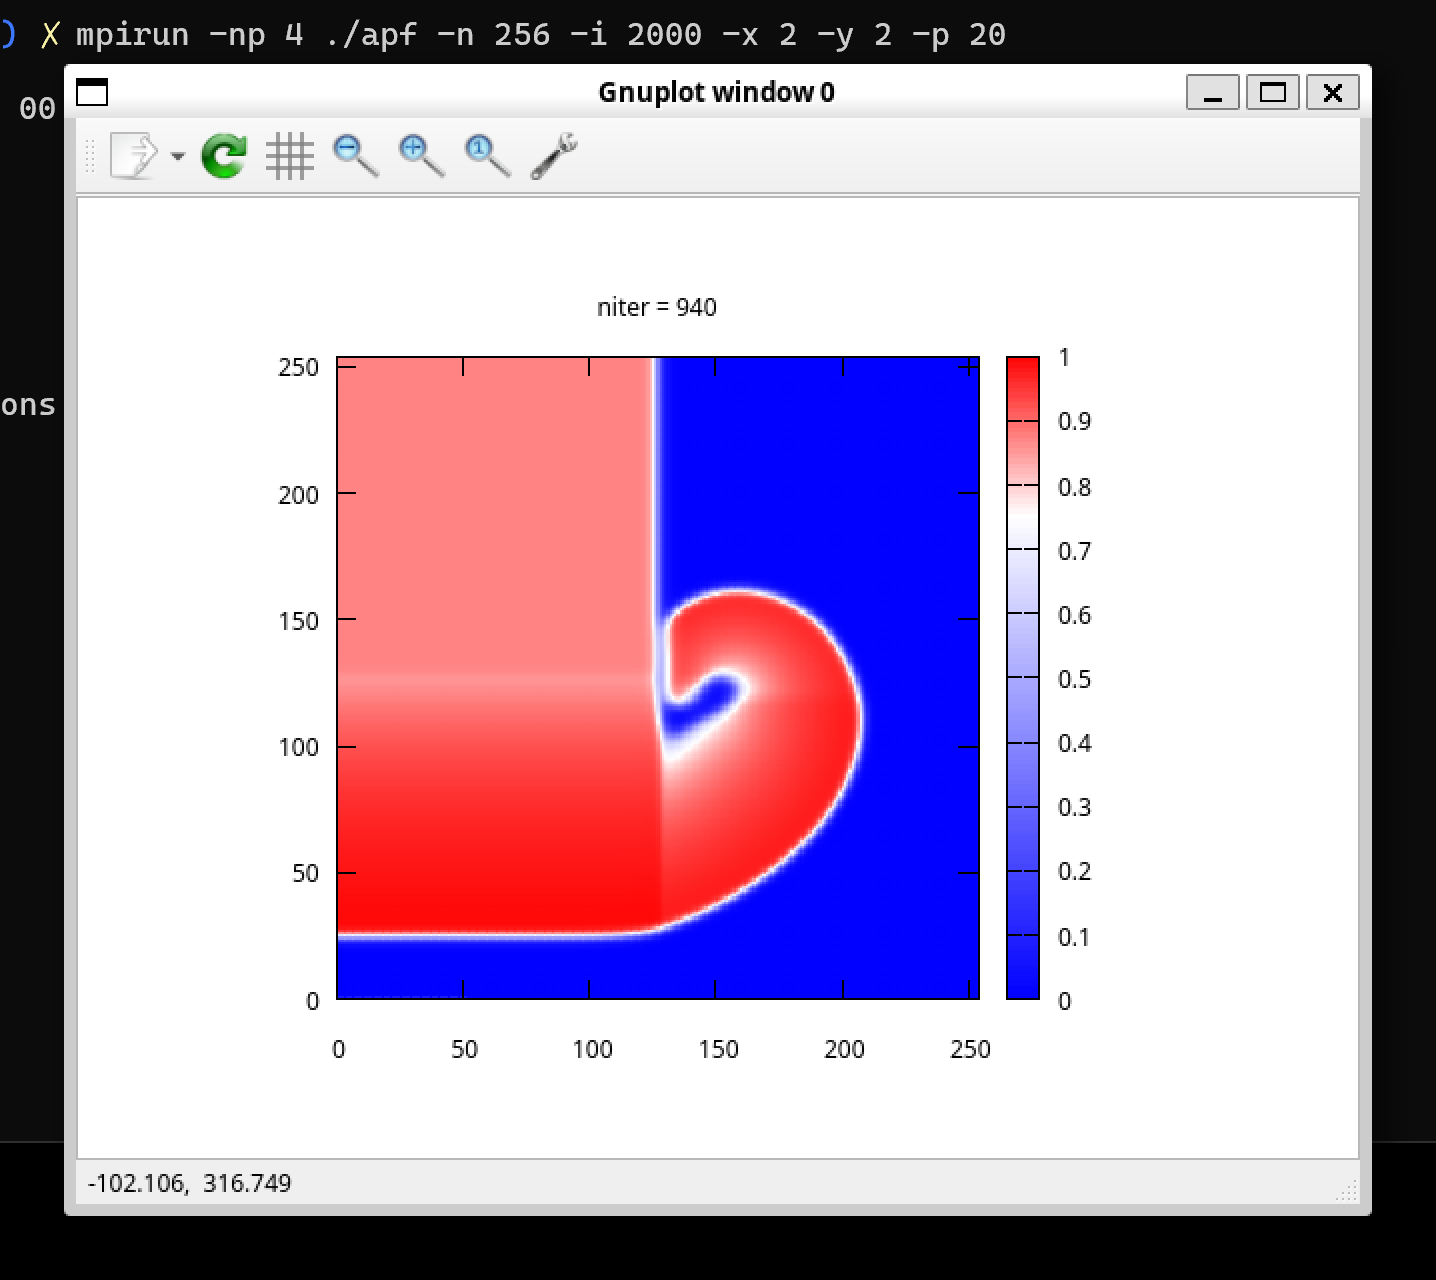
\includegraphics[width=\textwidth]{img/2.png}
    \end{minipage}
    \vfill
    \begin{minipage}[b]{0.45\textwidth}
        \centering
        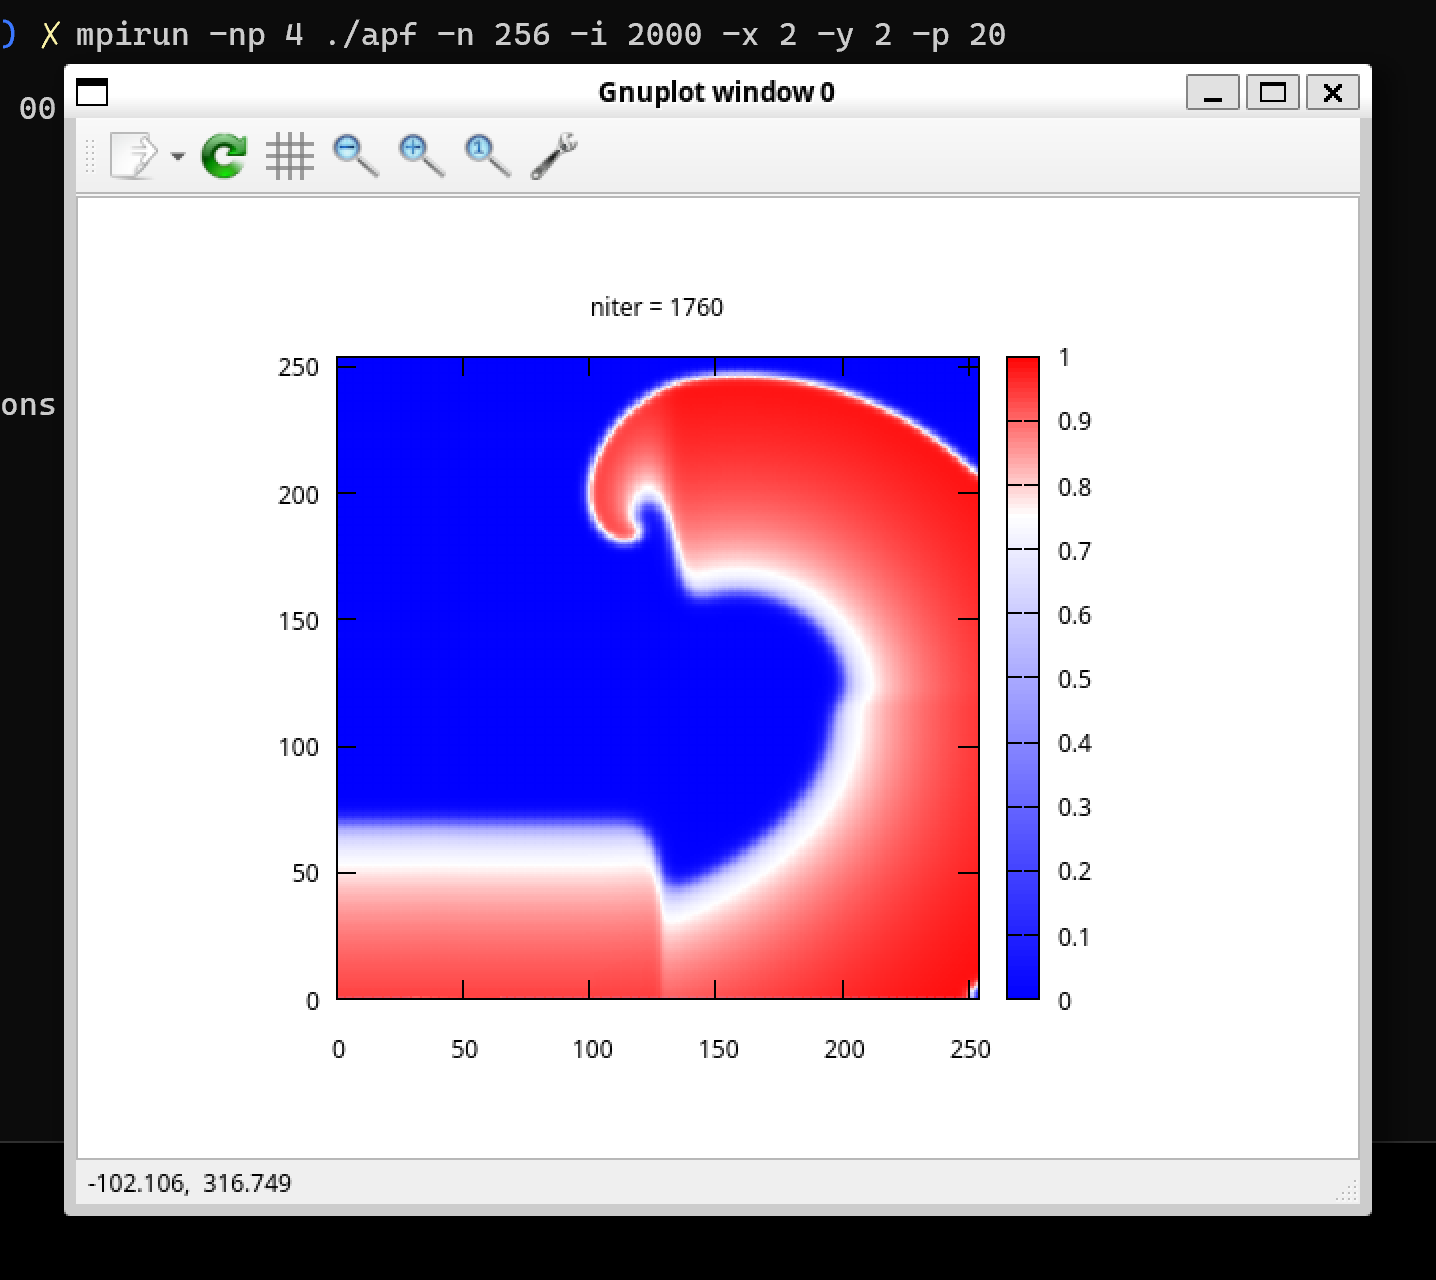
\includegraphics[width=\textwidth]{img/3.png}
    \end{minipage}
    \hfill
    \begin{minipage}[b]{0.45\textwidth}
        \centering
        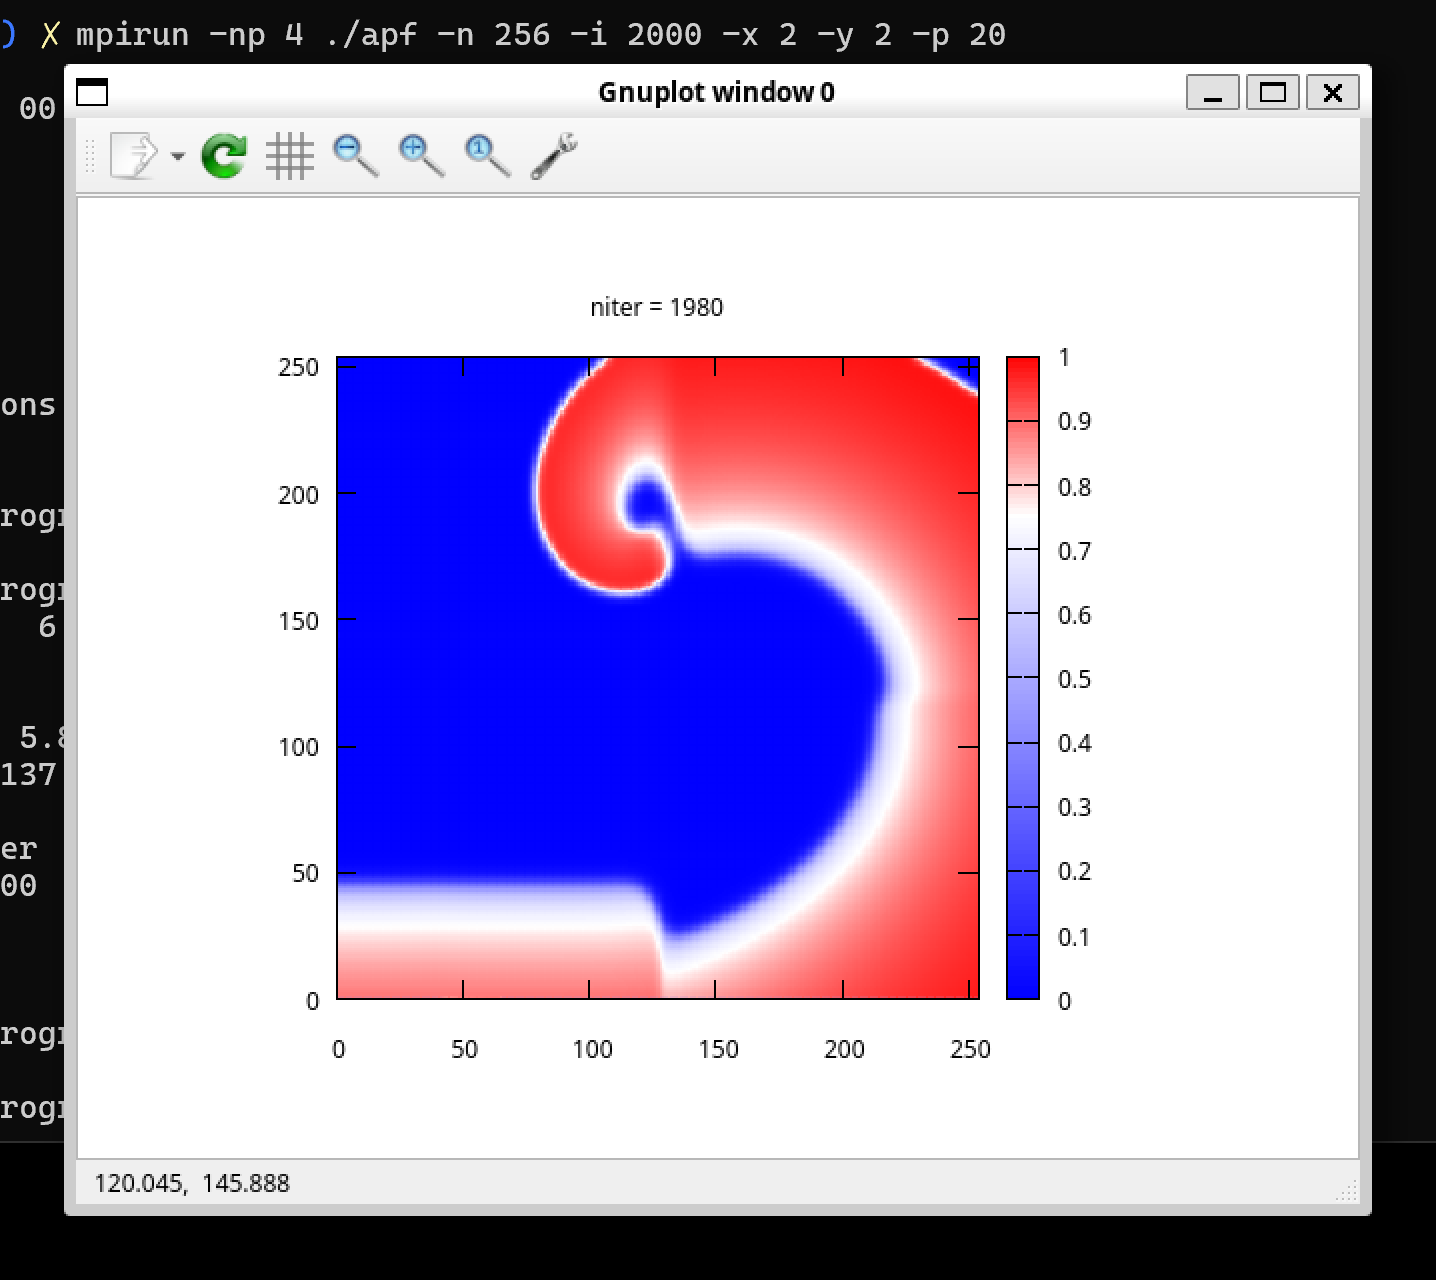
\includegraphics[width=\textwidth]{img/4.png}
    \end{minipage}
    \caption{live plot with 2x2 processes}
    \label{fig:images_grid}
\end{figure}

\subsection{vectorization}
The computation kernel and ghost cell exchange are vectorized.

\section{Potential Future Work}
% \textbf{What ideas did you have that you did not have a chance to try?}
\begin{enumerate}
    \item better distribution schedular to 
    distribute process on multiple CPUs and/or multiple nodes 
    and minimize the between-node communication.
    Essentially, break the full matrix into multiple level of sub matrices,
    and each computation unit (single processor, CPU die, node, server cluster, ...)
    takes their corresponding tasks based on this hierarchy. 
    \item investigate RDMA on and off performance differences.
\end{enumerate}

\end{document}
